\section{Introduction}

\begin{frame}
	\frametitle{Introduction}
	\vspace{-10ex}
	The root-locus method dealt with the s- and z-domain and the location of the poles and zeros formed the basis for that method.\\
	\medskip
	For the \textbf{frequency domain}, we use the following substitution: $s=j\omega$, which means we will only regard perfect oscillations.\\
	\medskip
	Sines, cosines and exponential signals are eigenfunctions of Linear Time Invariant systems (LTI).\\
	Perfect oscillations form the natural decomposition of each signal when you are dealing with LTIs.
\end{frame}

\begin{frame}
	\frametitle{Introduction}
	We need to translate our \textbf{design criteria} to something that fits the discussed method. For the root-locus method, we had to express the criteria in positions of poles and zeros.\\
	For the frequency domain, typical design criteria are:
	\begin{itemize}
		\item Phase and gain margin
		\item Bandwidth
		\item Zero-frequency magnitude (= DC gain)
	\end{itemize}
	\bigskip
	We will discuss two different \textbf{graphical representations} to design compensators in the frequency domain:
	\begin{itemize}
		\item Nyquist stability diagram and Nyquist plots
		\item Bode plots (for the design of lead, lag and lead-lag compensators)
	\end{itemize}
\end{frame}

\section{Stability}

\begin{frame}
	\frametitle{Stability of the closed loop system}
	\begin{figure}
		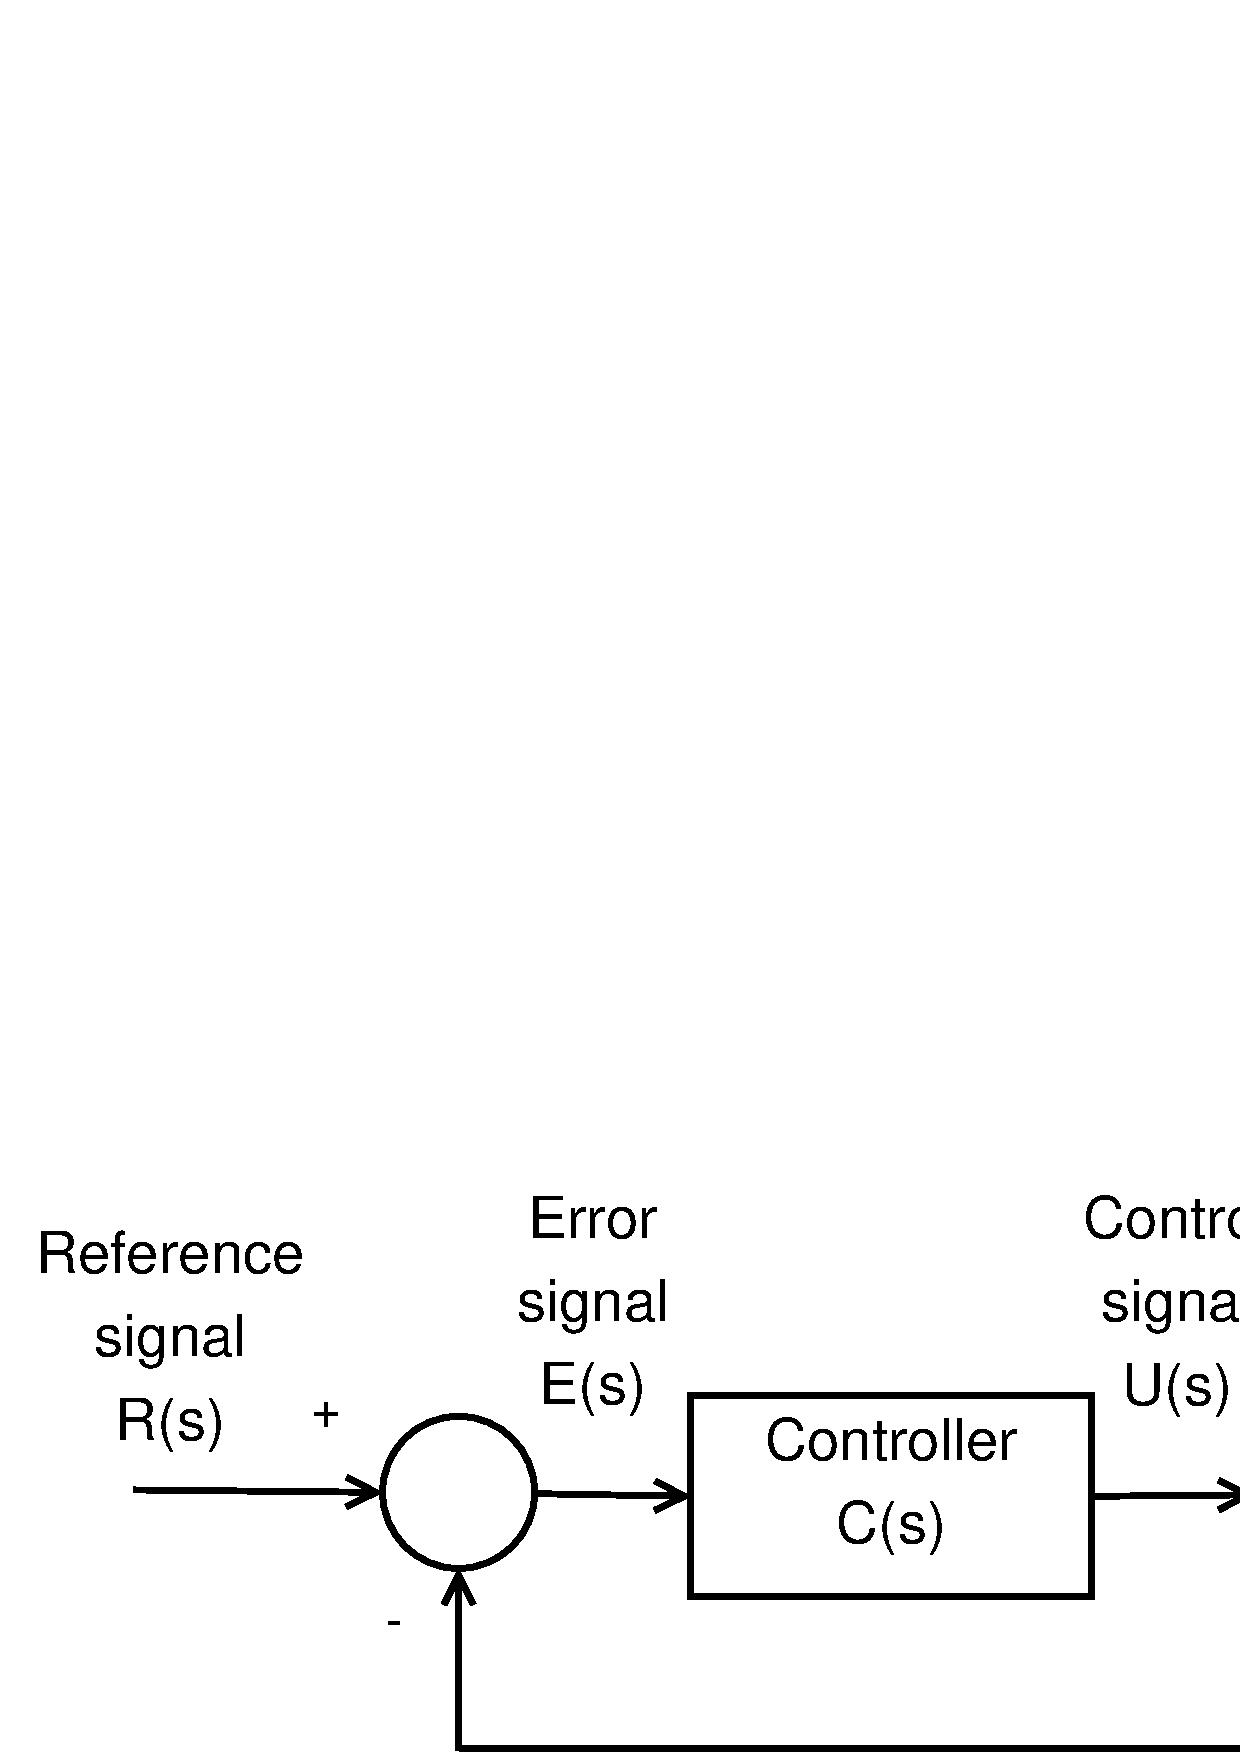
\includegraphics[width=0.8\linewidth]{closedloop}
	\end{figure}
	We write the output signal as a function of the input signal: $$Y(s)=\frac{P(s)C(s)}{1+P(s)C(s)}R(s).$$\\
	The closed loop system stability is determined by the poles of $\frac{P(s)C(s)}{1+P(s)C(s)}$, or the roots of $1+P(s)C(s)=0$.
\end{frame}

\begin{frame}
	\frametitle{Stability of the closed loop system}
	\vspace{-8ex}
	In the root-locus method, we determined the positions of the poles by plotting the roots of $1+P(s)C(s)=0$.\\
	\medskip
	The system is stable if all the roots remain in the left half plane.\\
	\medskip
	We are however not interested in the positions of the poles.\\
	We only need to know whether there are poles in the right half plane.\\
	\medskip
	There is a cheaper alternative: \textbf{the Nyquist stability criterion}.
\end{frame}

\begin{frame}
	\frametitle{Stability: Nyquist criterion}
	\vspace{-5ex}
	The Nyquist stability criterion avoids determining the roots of $1+P(s)C(s)$ exactly (expensive). It only determines the number of roots in the right half plane.\\
	\medskip
	It uses a theorem from complex calculus that finds the difference between the number of poles and the number of zeros within a contour (a closed curve).\\
	\medskip
	We will apply this theorem to $1+P(s)C(s)$ (which can be seen as a complex function) and the contour will encircle the entire right half plane (= the Nyquist contour).
\end{frame}

\section{Cauchy's argument principle}

\subsection{Complex function}

\begin{frame}
	\frametitle{Complex function}
	Before we get to the theorem, we discuss the concept of a complex function.\\
	\medskip
	A complex function $f(s)=u(x,y)+\mathit{j}v(x,y)$ maps the complex number $s=x+\mathit{j}y$ onto the complex number $w=u+\mathit{j}v$.
	\begin{columns}
		\column{0.5\textwidth}
		\begin{center}
			For a complex number:
		\end{center}
		\begin{figure}
			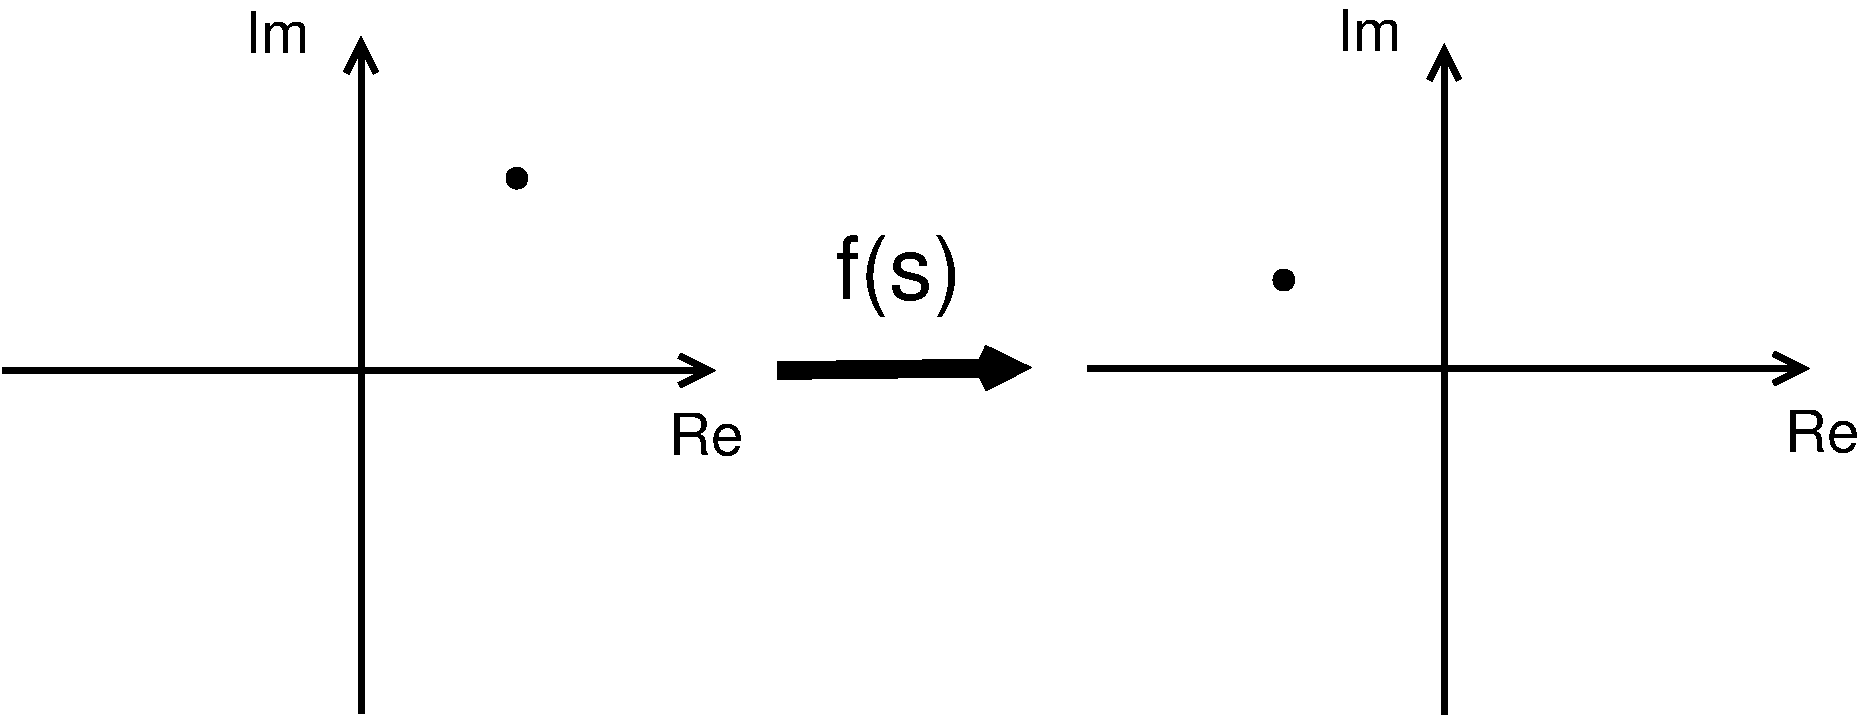
\includegraphics[width=1.0\linewidth]{complex1}
		\end{figure}
		\column{0.5\textwidth}
		\begin{center}
			or for a contour:
		\end{center}
		\begin{figure}
			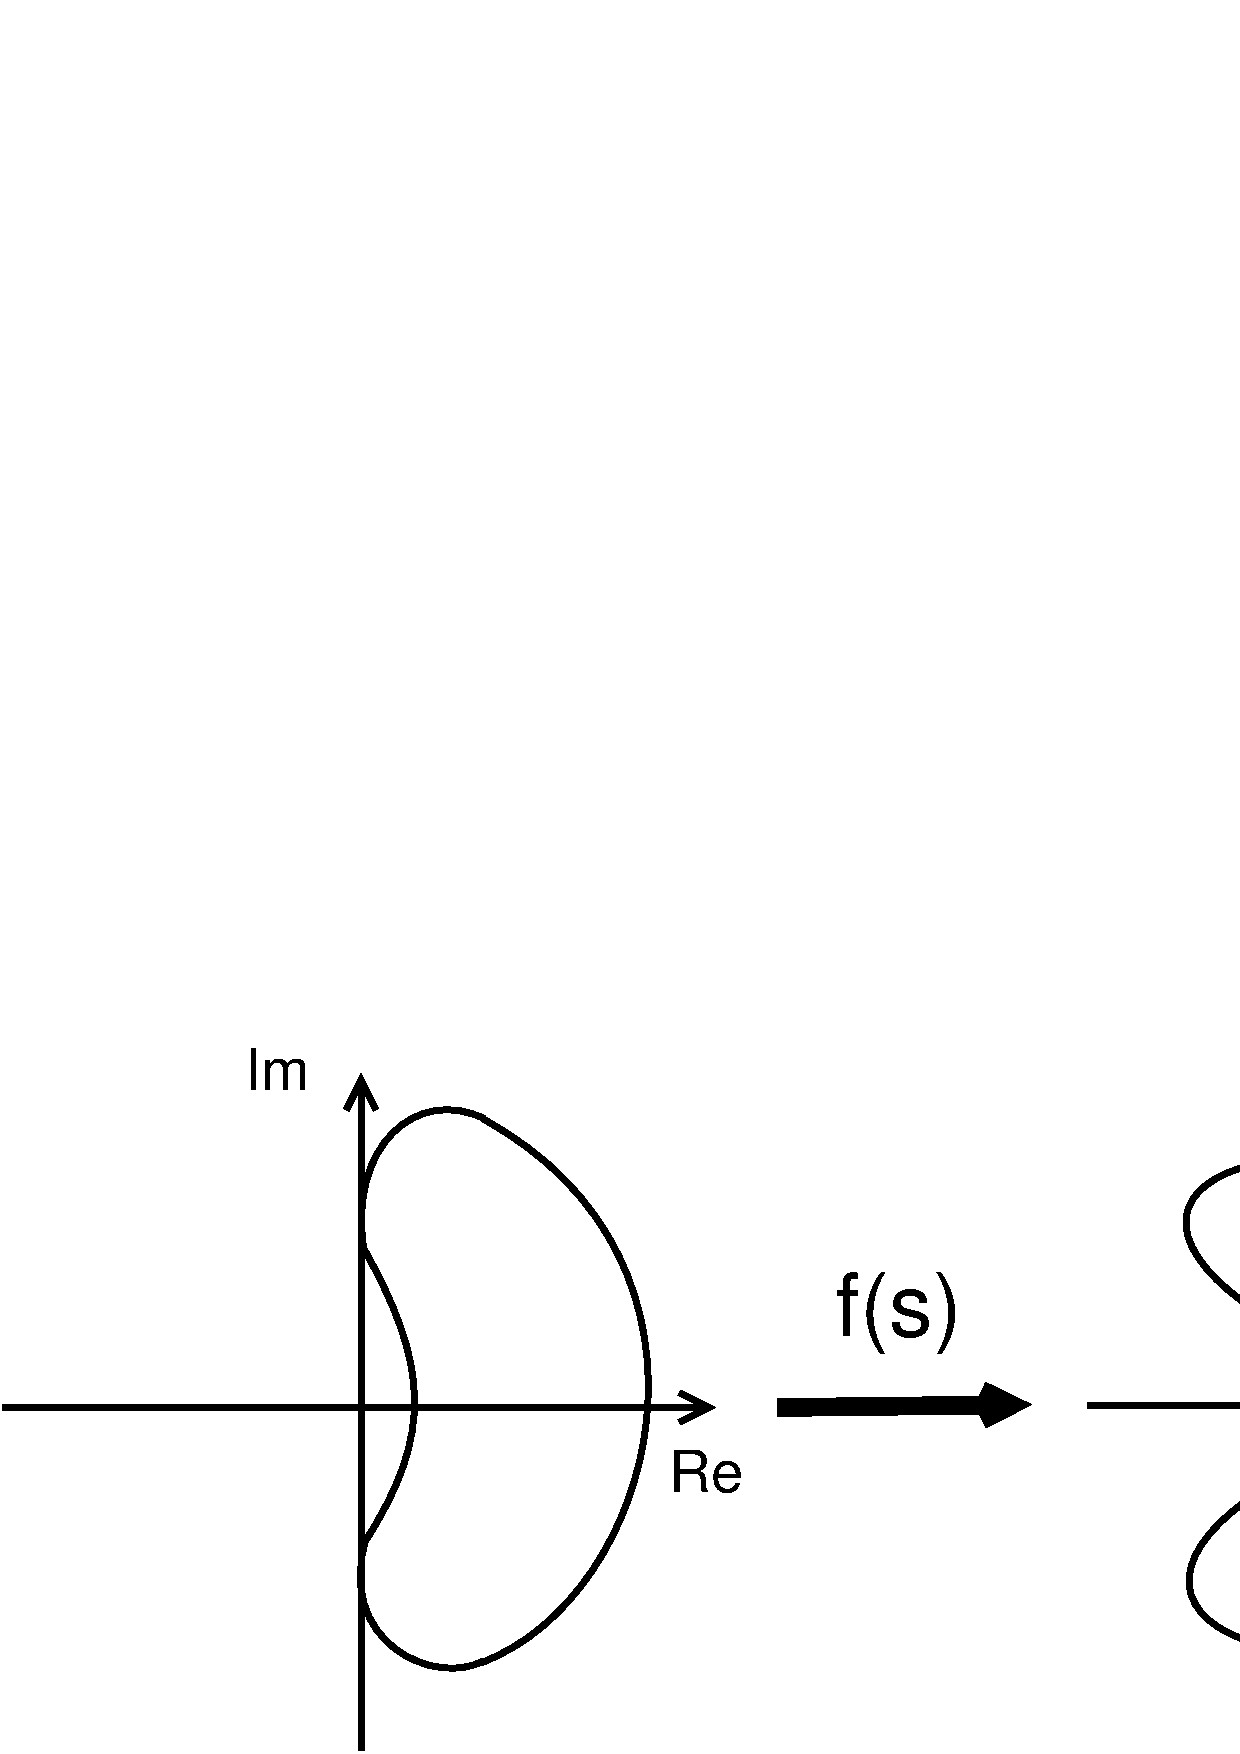
\includegraphics[width=1.0\linewidth]{complex2}
		\end{figure}
	\end{columns}
	\medskip
	The function $1+P(s)C(s)$ can also be regarded as a complex function, so we can use it as a mapping.
\end{frame}

\subsection{Cauchy's argument principle}

\begin{frame}
	\frametitle{Cauchy's argument principle}
	\vspace{-7ex}
	This is the engine behind the Nyquist stability criterion.\\
	\medskip
	If a contour $\Gamma$ in the s-plane circles Z zeros and P poles $f(s)$ in clockwise rotation, then the contour $\Gamma'$, which is the image of $\Gamma$ as mapped by $f(s)$, circles the origin (in the $\omega$-plane) Z-P times in the clockwise direction.\\
	\medskip
	So the only thing we are looking at is the encirclements of the origin. \\
	On the next slides, we will prove this.
\end{frame}

\begin{frame}
	\frametitle{Cauchy's argument principle}
	\vspace{-3ex}
	Let's take a complex function $f(s)=\frac{(s-z_1)(s-z_2)(s-z_3)...}{(s-p_1)(s-p_2)(s-p_3)...}$.\\
	\medskip
	If we would apply this function to a complex number c, this comes down to multiplying factors $c-z_i = A_{z_{i}}e^{j\theta_{z_{i}}}$ and $\frac{1}{c-p_i}=\frac{1}{A_{p_{i}}}e^{-j\theta_{p_{i}}}$.\\
	\medskip
	So the modulus of $f(c)$ can be easily found by evaluating $\frac{A_{z_{1}}A_{z_{2}}A_{z_{3}}...}{A_{p_{1}}A_{p_{2}}A_{p_{3}}...}$;\\
	\medskip
	This might help if you want to map a point, but it is not important for us.\\
	\medskip
	The evaluation of the argument of $f(c)$ is what will be interesting; $\angle f(c) = \theta_{z_{1}}+\theta_{z_{2}}+\theta_{z_{3}}+...-\theta_{p_{1}}-\theta_{p_{2}}-\theta_{p_{3}}-...$
\end{frame}

\begin{frame}
	\frametitle{Cauchy's argument principle: graphically}
	\begin{figure}
		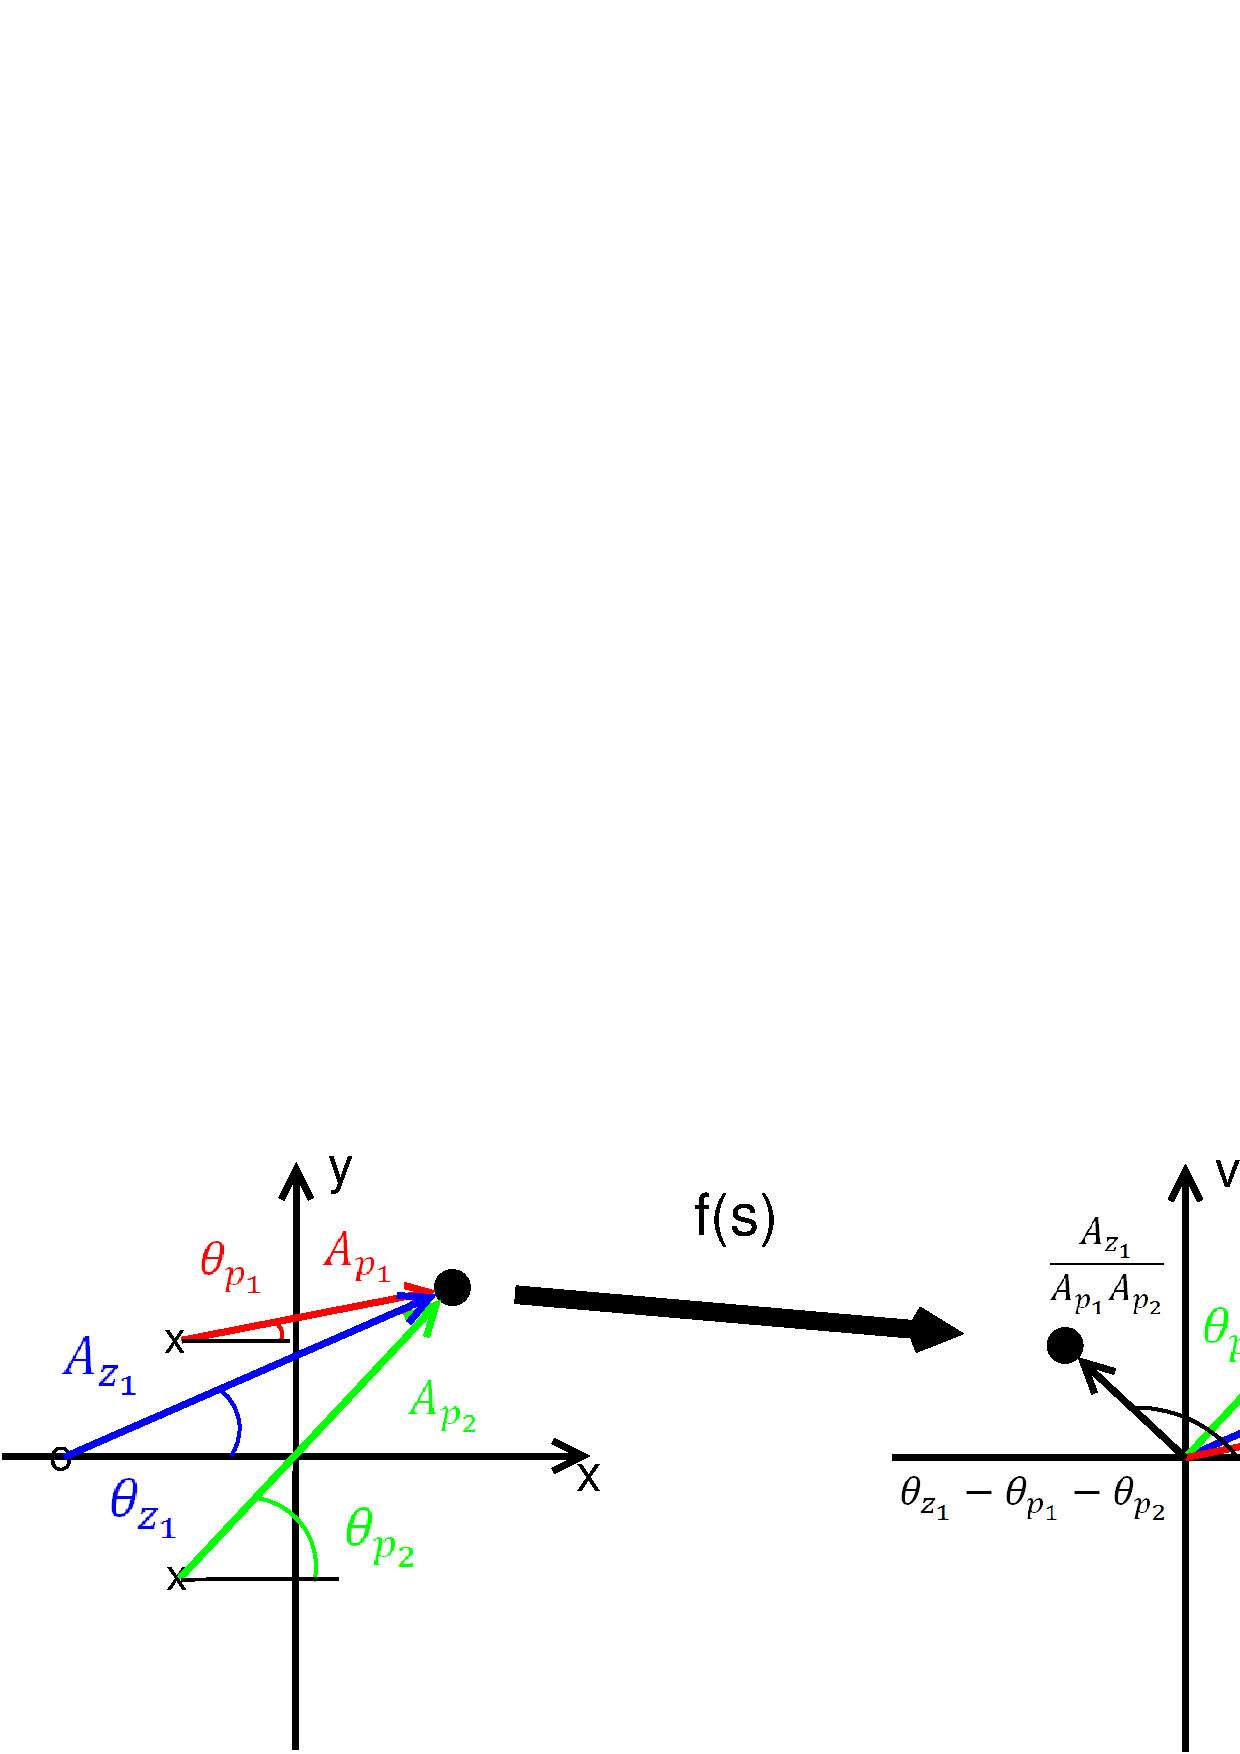
\includegraphics[width=1.0\linewidth]{graphical}
	\end{figure}
\end{frame}

\begin{frame}
	\frametitle{Cauchy's argument principle}
	When does the image of a contour in the $\omega$-plane encircle the origin?\\
	\medskip
	That happens when the argument of the image of the contour at the beginning and the end differ by $2\pi$.\\
	\medskip
	A pole or zero outside the contour will never have that effect. One inside the contour has the following effect:\\
	\medskip
	\begin{figure}
		
\includegraphics[width=1\linewidth]{argument}
	\end{figure}
\end{frame}

\begin{frame}
	\frametitle{Cauchy's argument principle}
	\vspace{-4ex}
	A pole results in $-2\pi$ (counterclockwise rotation), if the contour is followed clockwise.\\
	\medskip
	A zero results in $+2\pi$ (clockwise rotation).\\
	\medskip
	This follows from the sign of their effect: $\angle f(c) = \theta_{z_{1}}+\theta_{z_{2}}+\theta_{z_{3}}+...-\theta_{p_{1}}-\theta_{p_{2}}-\theta_{p_{3}}-...$\\
	\bigskip
	It is also possible that the origin is encircled when there are no poles or zeros in the contour (in the s-plane). But then the amount of clockwise encirclements equals the amount of counterclockwise encirclements hence no net encirclements.
\end{frame}

\subsection{Examples}

\begin{frame}
	\frametitle{Example 1}
	\begin{itemize}
		\item Two encircled poles (the x's): $P=2$
		\item Four encircled zeros (the o's): $Z=4$
		\item Hence: $N = Z-P = 2$
		\item Indeed, the image of the contour encircles the origin twice in the $\omega$-plane (in clockwise direction).
	\end{itemize}
	\begin{figure}
		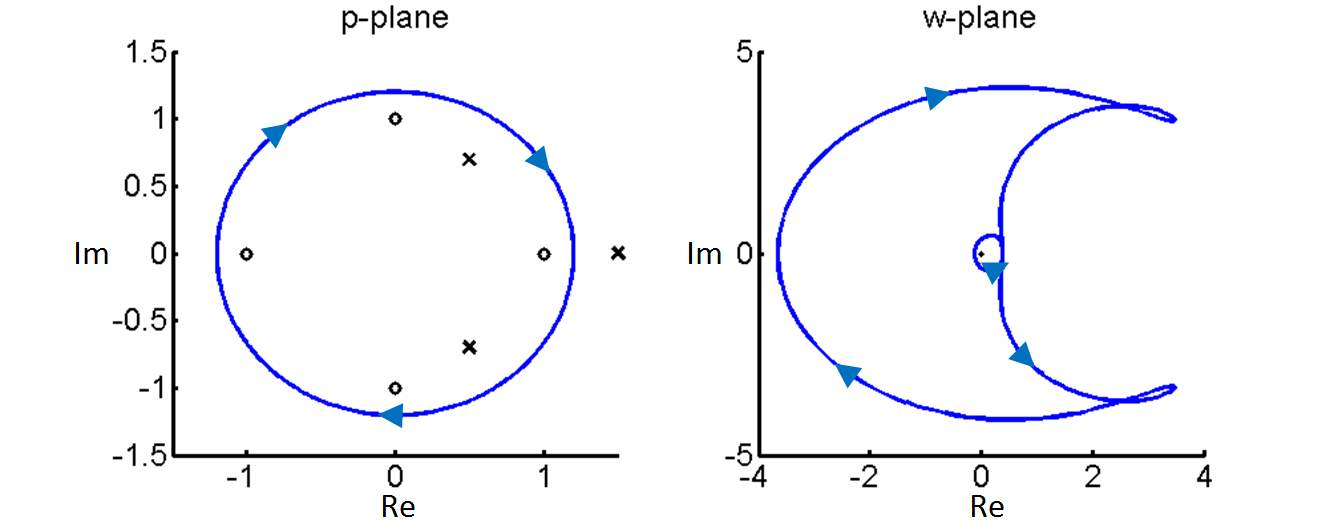
\includegraphics[width=1\linewidth]{example1}
	\end{figure}
\end{frame}

\begin{frame}
	\frametitle{Example 2}
	\begin{itemize}
		\item Two encircled poles: $P = 2$
		\item One encircled zero: $Z=1$
		\item Hence: $N=Z-P=-1$
		\item Indeed, the image of the contour encircles the origin once in the $\omega$-plane (in counterclockwise direction).
	\end{itemize}
	\begin{figure}
		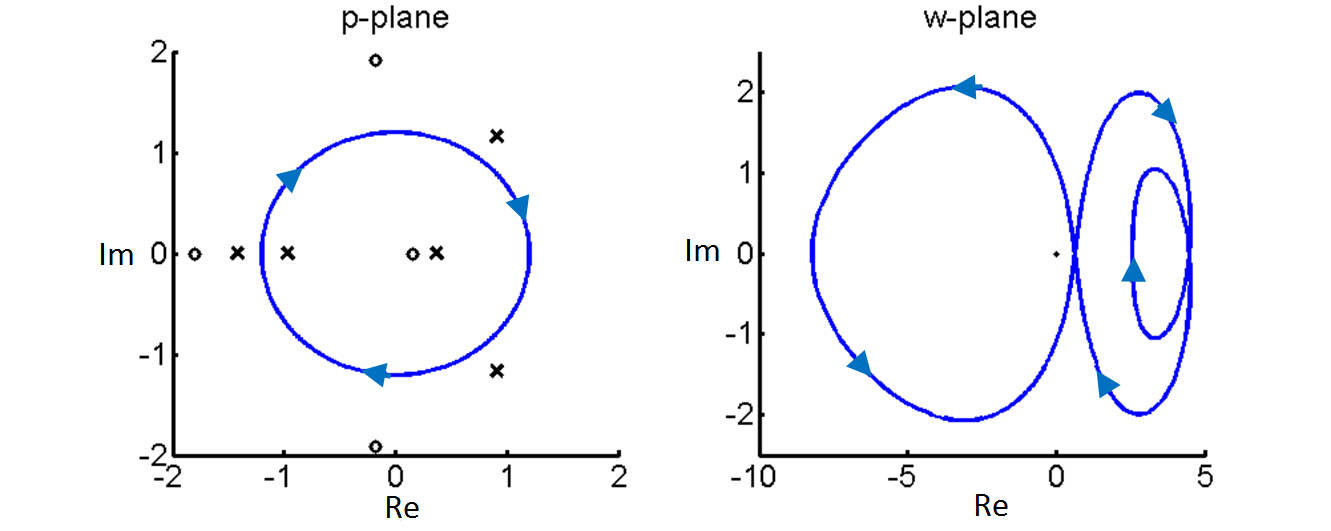
\includegraphics[width=0.8\linewidth]{example2}
	\end{figure}
\end{frame}

\section{Nyquist stability criterion}

\subsection{Nyquist stability criterion}

\begin{frame}
	\frametitle{Nyquist stability criterion}
	If we apply Cauchy's argument principle to the following contour (the Nyquist contour), the amount of clockwise encirclements around the origin of the image of this contour (called the Nyquist plot) in the $\omega$-plane equals $Z-P$ of the right half plane (RHP).
	\begin{figure}
		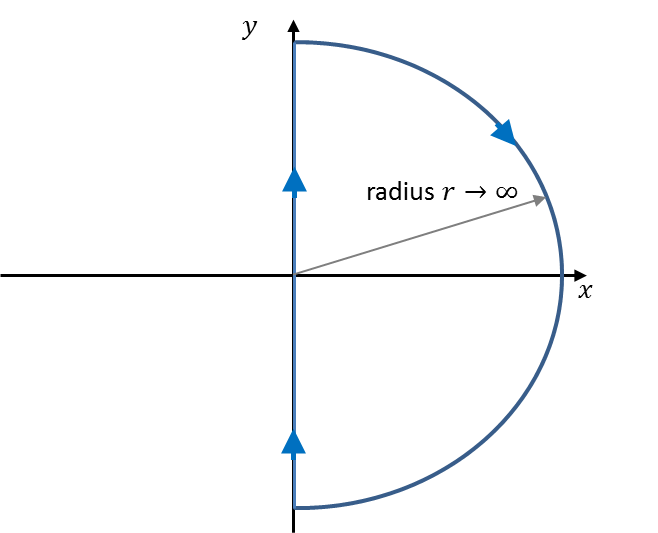
\includegraphics[width=0.55\linewidth]{nyquist}
	\end{figure}
\end{frame}

\begin{frame}
	\frametitle{Nyquist stability criterion}
	That way we will find the difference between the number of poles and zeros of $1+P(s)C(s)$ in the RHP: $N=Z-P$.\\
	\medskip
	So if we know P (the number of poles in the RHP of $1+P(s)C(s)$), we know how many zeros of $1+P(s)C(s)$ there are in the RHP.
	\begin{figure}
		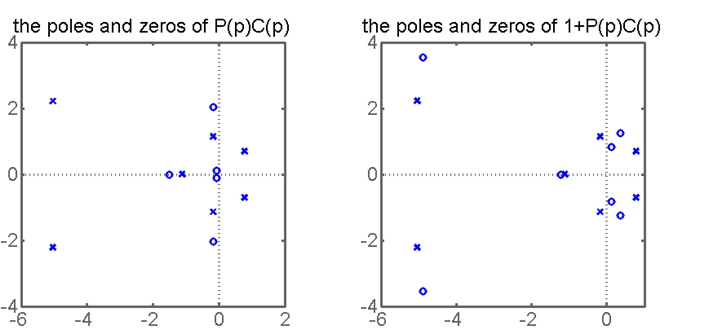
\includegraphics[width=0.8\linewidth]{pz}
	\end{figure}
\end{frame}

\begin{frame}
	\frametitle{Nyquist stability criterion}
	\vspace{-10ex}
	Luckily this last aspect is simple, since the poles of $1+P(s)C(s)$ equal those of $P(s)C(s)$. Hence the amount of RHP poles is equal (the connection between the zeros is not clear).\\
	\bigskip
	So if we assume the number of RHP poles of $P(s)C(s)$ is known (which we'll assume), we know whether the system with unity (negative) feedback is stable.
\end{frame}

\begin{frame}
	\frametitle{Nyquist stability criterion}
	If we apply this to $1+P(s)C(s)$, we need to count the number of encirclements of the origin.\\
	However, the Nyquist stability criterion uses $P(s)C(s)$.
	\begin{itemize}
		\item The zeros of $1+P(s)C(s)$ and the poles and zeros of $P(s)C(s)$ are hard to relate.
		\item This is in sharp contrast with how easily the Nyquist plots relate.
		\item The Nyquist plot of $P(s)C(s)$ equals the one of $(1+P(s)C(s)$, after it has been moved to the right over a distance 1.
		\item To find $Z-P$, one has to count the number of clockwise encirclements of the image of $P(s)C(s)$ around the point $(-1,0)$, since this equals the number of clockwise encirclements of the image of $1+P(s)C(s)$ around the origin.
	\end{itemize}
\end{frame}

\begin{frame}
	\frametitle{Nyquist stability criterion}
	\begin{block}{Nyquist stability criterion}
		If the open loop system $P(s)C(s)$ has $\ell$ poles in the open right half plane (of the s-plane),\\
		then the system with unity feedback is stable if and only if the Nyquist plot encircles the point (-1,0) $\ell$ times in the counter clockwise direction.
		\end{block}
\end{frame}

\subsection{Nyquist plot}

%SLIDE 23 IN VOORLOPIGE VERSIE

%%---------------------------------------------------OLD SLIDES---------------------------------------------------

%\begin{frame}
%\frametitle{Moving to the frequency domain}
%\begin{itemize}
%\item The root locus method dealt with the $s$ and the $z$ domain and the
%location of the poles and zeros formed the basis of that method
%\vspace{1.5cm}
%\item Now we go to the frequency domain: $s=j\omega$ which means
%we will only regard perfect oscillations
%\end{itemize}
%\end{frame}
%
%\begin{frame}{Moving to the frequency domain}
%\begin{itemize}
%\item This cannot be seen apart from the fact that \\sines, cosines
%and exponential signals are eigenfunctions of Linear Time Invariant (LTI) systems
%\vspace{1.5cm}
%\item Perfect oscillations form the natural decomposition of each
%signal when you are dealing with LTI's
%\end{itemize}
%\end{frame}
%
%\begin{frame}
%\frametitle{Design criteria}
%\begin{itemize}
%\item Like before, we need to translate our design criteria into a language that fits the discussed method
%\vspace{1cm}
%\item For the root-locus method that meant that we had to express our criteria in positions of poles and zeros
%\vspace{1cm}
%\item Typical design criteria in the frequency domain are: \begin{itemize}
%\vspace{0.25cm}
%\item Phase and gain margin: their meaning will be discussed thoroughly in the section about the Nyquist stability criterion
%\vspace{0.5cm}
%\item Bandwidth: this will be discussed when we tackle Bode plots
%\vspace{0.5cm}
%\item Zero-frequency magnitude (= DC gain)
%\end{itemize}
%\end{itemize}
%\end{frame}
%
%\begin{frame}
%\frametitle{Design tools}
%\begin{itemize}
%\vspace{-1cm}
%\item We will use two different graphical representations to design compensators in the frequency domain:
%\\ \begin{itemize}
%\vspace{0.75cm}
%\item First we will introduce the Nyquist stability diagram and Nyquist plots
%\vspace{0.75cm}
%\item When we discuss the design of lead, lag and lead-lag compensators we will use Bode plots (frequency domain design tool)
%\end{itemize}
%\end{itemize}
%\end{frame}
%
%\begin{frame}
%\frametitle{Nyquist stability criterion: what and why?}
%\begin{itemize}
%\vspace{-0.25cm}
%\item What?\\
%\vspace{0.35cm}
%The Nyquist stability criterion is a way of determining the stability of a closed loop linear time-invariant system based on the open loop system
%\vspace{0.25cm}
%\item Why is it useful?\\
%\vspace{0.35cm}
%It is cheap to compute
%It allows to determine the phase and gain margins
%\vspace{0.25cm}
%\item Do we have what it takes?\\
%\vspace{0.35cm}
%In order to use it, you need to know the number of right half plane poles of the open loop system; which you usually know
%The calculations simplify significantly for a physically realizable system
%\end{itemize}
%\end{frame}
%
%\begin{frame}
%\frametitle{Nyquist stability criterion: what and why?}
%\begin{itemize}
%\vspace{-1.5cm}
%\item It was discovered in $1932$ in order to have a cheaper method of determining stability (back then finding the roots of $1+P(s)C(s)$ was a very expensive endeavor)\\
%\vspace{2.5cm}
%\item Now it is still relevant as a design tool
%\end{itemize}
%\end{frame}
%
%\begin{frame}
%\frametitle{Stability of the closed loop system}
%\begin{itemize}
%\item The closed loop system stability is determined by the poles of $\frac{P(s)C(s)}{1+P(s)C(s)}$, or the roots of $1+P(s)C(s)=0$
%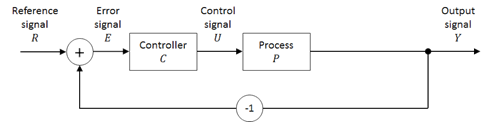
\includegraphics{Afbeelding1}
%\item In the root locus method we determined the position of the poles by plotting the roots of $1+P(s)C(s)=0 $ thus finding whether it is stable by checking whether all the roots remain in the left half plane
%\item Solving $1+P(s)C(s)=0$ was very expensive $50$ years ago
%\item We are not interested in the position of the poles. The only thing we need to know is whether there are poles in the right half plane or not. We can find a cheaper alternative, the Nyquist stability criterion
%\end{itemize}
%\end{frame}
%
%\begin{frame}
%\frametitle{Stability of the closed loop system: Nyquistcriterion}
%\begin{itemize}
%\item The Nyquist stability criterion avoids determining the roots of $1+P(s)C(s)$ exactly, it only determines the number of roots in the right half plane
%\item It uses a theorem from complex calculus that finds the difference between the number of poles and the number of zeros within a contour (a closed curve)
%\item We will apply this theorem to $1+P(s)C(s)$ (which can be seen as a complex function) and the contour will encircle the entire right half plane (= the Nyquistcontour)
%\end{itemize}
%\end{frame}
%
%\begin{frame}
%\frametitle{Complex function}
%\begin{itemize}
%\item Before we get to the theorem that allows us to determine $Z-P$ (the number of zeros minus the number of poles within a contour), we have to show what a complex function is
%\item A complex function $f(s)= u(x,y) +jv(x,y)$ maps the complex number $s= x+jy$ onto the complex number $w= u+jv$ \\
%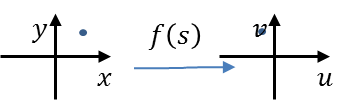
\includegraphics{Afbeelding2} \\or for a contour:\\ 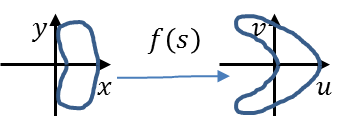
\includegraphics{Afbeelding3}
%\item The function $1+P(s)C(s)$ can also be regarded as a complex function, so we can use it as a mapping
%\end{itemize}
%\end{frame}
%
%\begin{frame}
%\frametitle{Cauchy's argument principle}
%\begin{itemize}
%\item This is the engine behind the Nyquist stability criterion
%\item If a contour $\Gamma$ in the $s$-plane circles $Z$ zeros and $P$ poles of $f(s)$ in clockwise (CW) rotation, then the contour $\Gamma'$, which is the image of $\Gamma$ as mapped by $f(s)$, circles the origin (in the $w$-plane) $Z-P$ times in the clockwise (CW) direction
%\item So the only thing we are looking at is the encirclements of the origin, all the other wiggles don’t matter to us
%\item On the next slides we will prove this
%\item If you want to know more about this and related topics, we refer you to the course 'Complexefunctieleer–1stmaster WIT'
%\end{itemize}
%\end{frame}
%
\begin{frame}
\frametitle{Cauchy’s argument principle}
\begin{itemize}
\item Let’s take a complex function $f(s)=\frac{(s-z_1)(s-z_2)(s-z_3)...}{(s-p_1)(s-p_2)(s-p_3)...}$ 
\item So if we would apply this function to a complex number c then this comes down to multiplying factors $ c-z_1 = A_{z_1}e^{j\theta_{z_1}}$ and $\frac {1}{c-p_1} = \frac{1}{A_{p_1}}e^{-j\theta_{p_1}} $ 
\item So the modulus of $f(c)$ can be easily found by evaluating $\frac{A_{z_1}A_{z_2}A_{z_3}...}{A_{p_1}A_{p_2}A_{p_3}...}$ ;this might help if you want to map a point, but it is not important for us.
\item The evaluation of the argument of $f(c)$ is what will be interesting; it is also very easy to find: $ \angle f(c) = \theta_{z_1} + \theta_{z_2}+\theta_{z_3}+...-\theta_{p_1} - \theta_{p_2} - \theta_{p_3}-... $ 
\end{itemize}
\end{frame}

\begin{frame}
\frametitle{Cauchy’s argument principle}
Let’s first show this graphically:

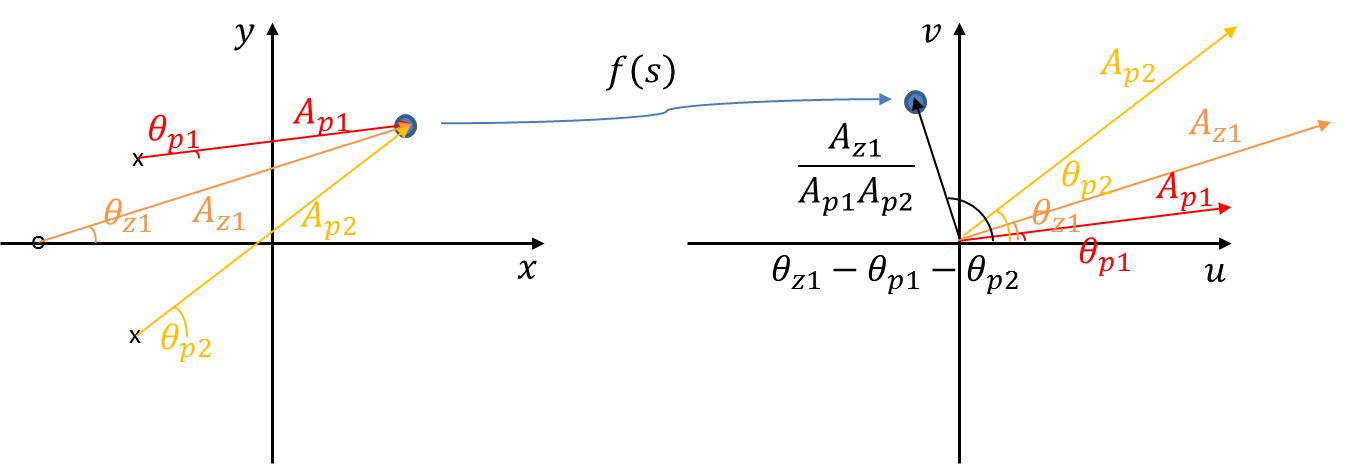
\includegraphics[width= 0.9\linewidth]{Afbeelding4} 
\end{frame}

\begin{frame}
\frametitle{Cauchy’s argument principle}
\begin{itemize}
\item When does the image of a contour in the $w$-plane encircle the origin?
\item That happens when the image of the beginning and the end of the contour their argument differs by $2\pi$
\item A pole/zero outside the contour will never have that effect and one inside the contour does:
\\
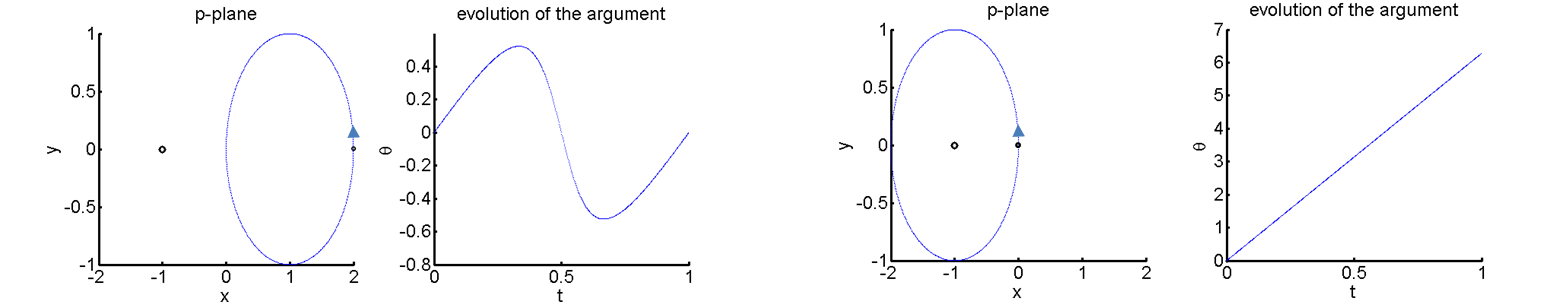
\includegraphics[width=0.95\linewidth]{Afbeelding5}
\end{itemize}
\end{frame}

\begin{frame}
\frametitle{Cauchy’s argument principle}
\begin{itemize}
\item A pole results in $-2\pi$ (CCW rotation), if the contour is followed CW, and a zero results in $+2\pi$ (CW rotation) follows from the sign of their effect: \\$ \angle f(c) = \theta_{z_1} + \theta_{z_2}+\theta_{z_3}+...-\theta_{p_1} - \theta_{p_1} - \theta_{p_1}-... $ 
\item Watch out: it is also possible that the origin is encircled when there are no poles or zeros in the contour (in the $s$-plane); but then the amount of CW encirclements equals the amount of CCW encirclements hence no net encirclements
\end{itemize}
\end{frame}

\begin{frame}
\frametitle{Cauchy’s argument principle: examples}
\begin{itemize}
\item Two encircled poles (the x' s): $P=2$
\item Four encircled zeros (the o' s): $Z=4$
\item Hence: $N= Z-P= 2$
\item Indeed, the image of the contour encircles the origin twice in the $w$-plane (in the CW direction)
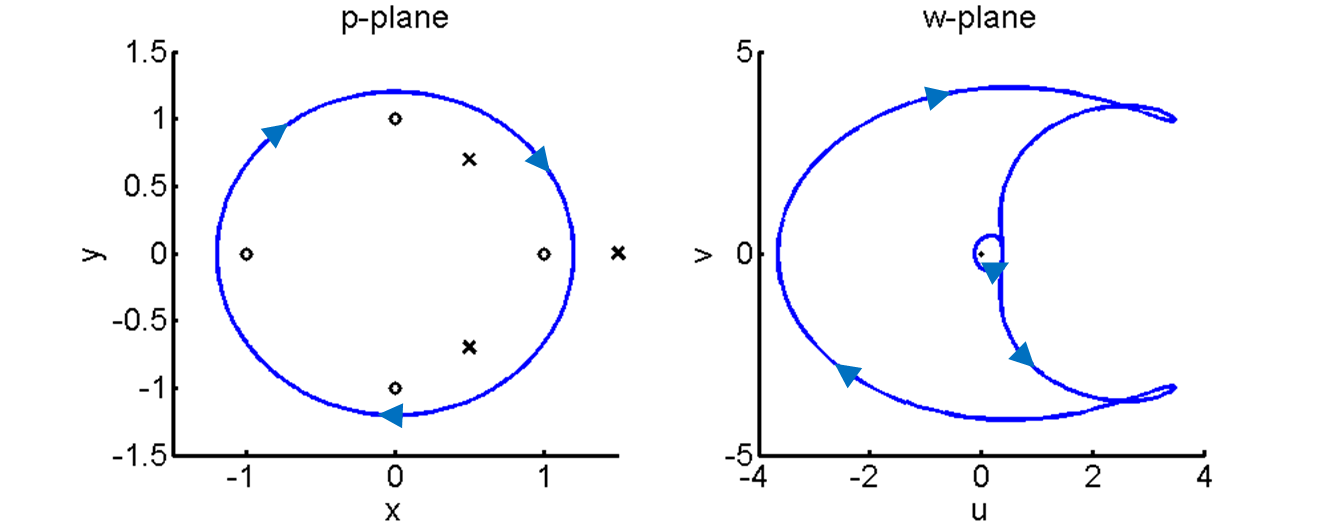
\includegraphics[width=0.9\linewidth]{Afbeelding6}
\end{itemize}
\end{frame}

\begin{frame}
\frametitle{Cauchy’s argument principle: examples}
\begin{itemize}
\item Two encircled poles (the x' s): $P=2$
\item Four encircled zeros (the o' s): $Z=1$
\item Hence: $N= Z-P= -1$
\item Indeed, the image of the contour encircles the origin once in the w-plane (in the CCW direction)
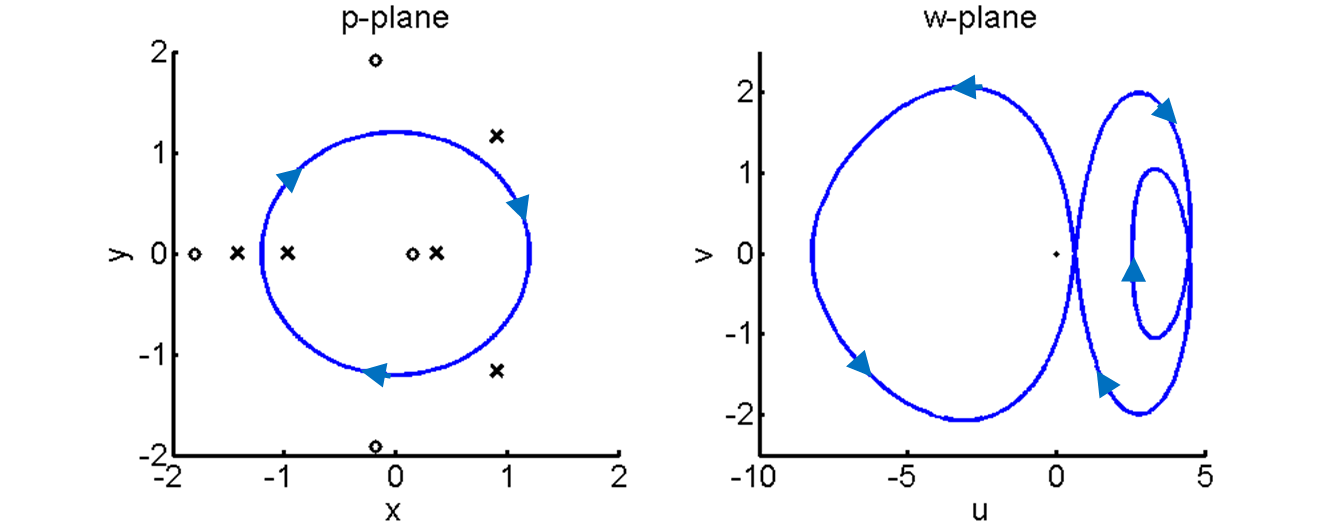
\includegraphics[width=0.9\linewidth]{Afbeelding7}
\end{itemize}
\end{frame}

\begin{frame}
\frametitle{Nyquist stability criterion}
 If we apply Cauchy’s argument principle to the following contour (the Nyquistcontour), the amount of CW encirclements around the origin of the image of this contour (called the Nyquist plot) in the $w$-plane equals $Z-P$ of the RHP\\
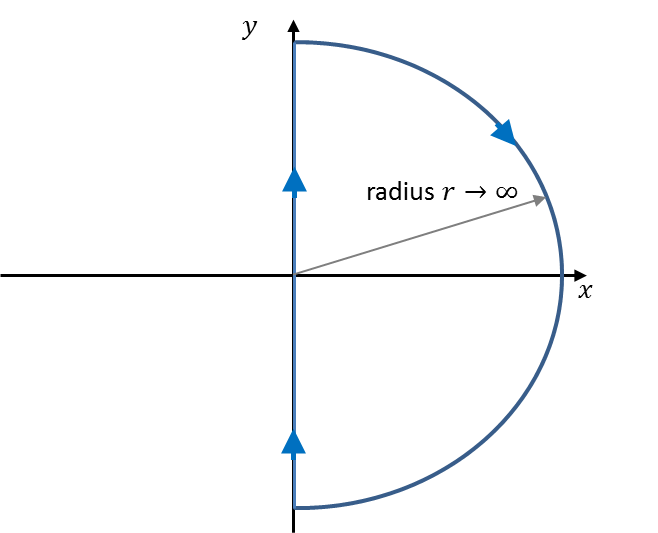
\includegraphics[width=0.7\linewidth]{Afbeelding8}
\end{frame}

\begin{frame}
\frametitle{Nyquist stability criterion}
\begin{itemize}
\item That way we will find the difference between the number of poles and zeros of $1+P(s)C(s)$ in the RHP: $ N= Z-P $
\item So if we now know $P$ (the number of poles in the RHP of $1+P(s)C(s)$ ), we can know whether (and how many) zeros of $1+P(s)C(s)$ are in the RHP\\
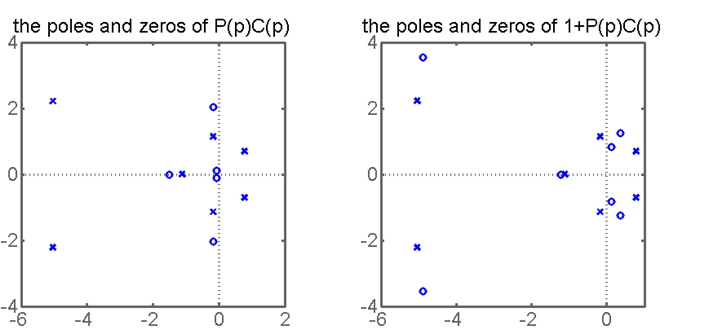
\includegraphics[width=0.8\linewidth]{Afbeelding9}
\end{itemize}
\end{frame}

\begin{frame}
\frametitle{Nyquist stability criterion}
\begin{itemize}
\item Luckily this last aspect is simple; since the poles of $1+P(s)C(s)$ equal those of $P(s)C(s)$; hence the amount of RHP poles is equal \\(the connection between the zeros is not clear)
\item So if we assume the number of RHP poles of $P(s)C(s)$ is known (which we'll assume), we can know whether the system with unity feedback is stable
\end{itemize}
\end{frame}

\begin{frame}
\frametitle{Nyquist stability criterion}
So we could apply this to $1+P(s)C(s)$, then the encirclements of the origin counts indeed
\\But the Nyquist stability criterion applies this to $P(s)C(s)$
\begin{itemize} 
\item We saw that the zeros of $1+P(s)C(s)$ and the poles and zeros of $P(s)C(s)$ are hard to relate.
\item This is in sharp contrast with how easily the Nyquist plots relate
\item The Nyquist plots of $P(s)C(s)$ equals the one of $1+P(s)C(s)$, after he has been moved $1$ to the right
\item So to find $Z-P $ one has to count the number of CW encirclements of the image of $P(s)C(s)$ around ($-1$,$0$) since this equals the number of CW encirclements of the image of $1+P(s)C(s)$ around the origin.
\end{itemize}
\end{frame}

\begin{frame}
\frametitle{Nyquist stability criterion}
Nyquist stability criterion:
\\ \fbox{\parbox{\textwidth}{%
If the open loop system $P(s)C(s)$ has $l$-poles in the open right half plane (of the $s$-plane),\\ then the system with unity feedback is stable if and only if the Nyquist plot encircles the point\\ ($-1$,$0$) $l$ times in the counter clockwise direction}}
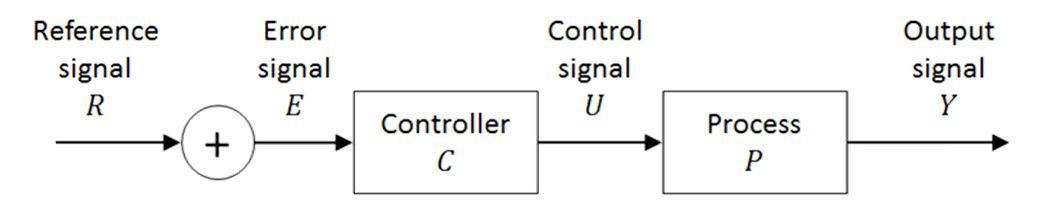
\includegraphics[width=0.7\linewidth]{Afbeelding10}
\\ 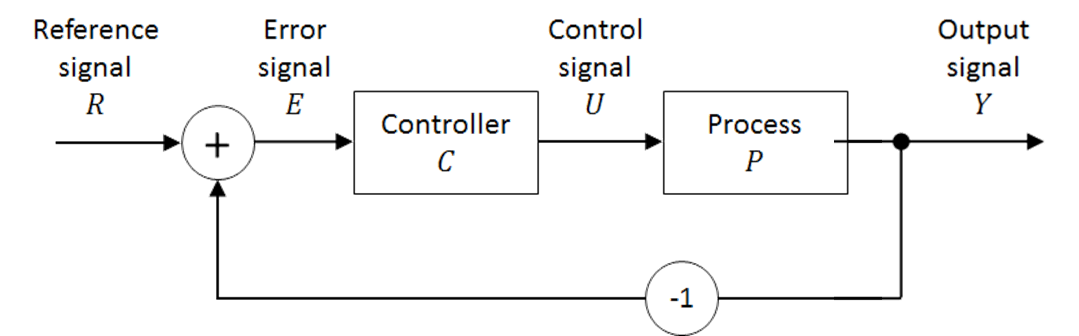
\includegraphics[width=0.7\linewidth]{Afbeelding11}
\end{frame}

\begin{frame}
\frametitle{Nyquist plot }
We now found how to deduce stability of the closed loop system from the Nyquist plot
\\
Now we will discuss how these plots can be found
\\
But first some simplifications:
\begin{itemize}
\item For physically realizable systems (i.e. relevant systems to engineers) the circle bow will be mapped on a point
\item The image of the positive imaginary axis is the mirror image of the image of the negative imaginary axis
\\ 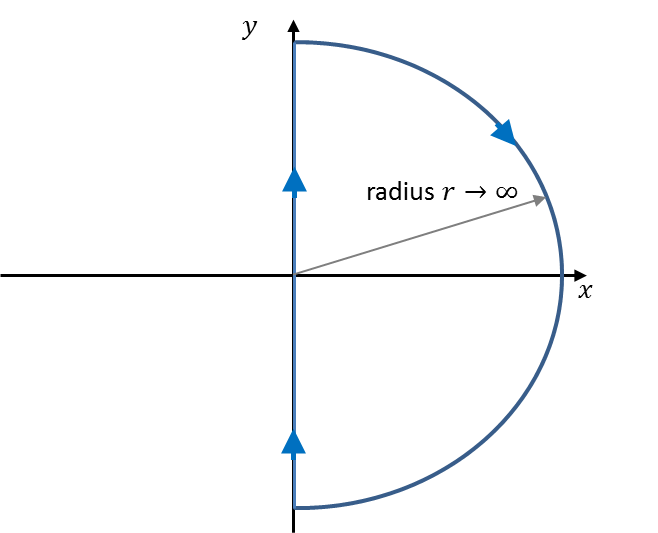
\includegraphics[width=0.5
\linewidth]{Afbeelding8}
\end{itemize}
\end{frame}

\begin{frame}
\frametitle{Nyquist plot: physically realizable systems}
\begin{itemize}
\item Where does the very convenient property of physically realizable systems come from?
\item The reason is:\begin{enumerate}
\item Every physically realizable system is causal
\item Every causal system has a transfer function with an order of the denominator that is larger than or equal to the order of the numerator
\item From this shape of the transfer function we can easily show that the circle bow maps onto a point
\\ 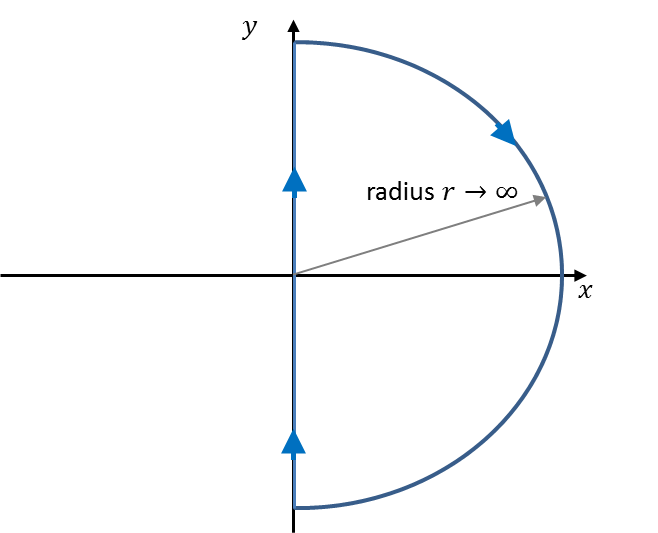
\includegraphics[width=0.5
\linewidth]{Afbeelding8}
\end{enumerate}
\end{itemize}
\end{frame}


\newcounter{sauvegardeenumi}
\newcommand{\asuivre}{\setcounter{sauvegardeenumi}{\theenumi}}
\newcommand{\suite}{\setcounter{enumi}{\thesauvegardeenumi}}


\begin{frame}
\frametitle{Nyquist plot: physically realizable systems}
\begin{enumerate}
\item Every physically realizable system is causal
\\This is logical: you cannot build a system that knows the future
\item Every causal system has a transfer function with an order of the denominator that is larger than or equal to the order of the numerator
\\This can be easily understood in the discrete time case:
\\ $ a_0y_n + a_1y_{n-1} + a_2y_{n-2} + ... = b_ou_n + b_1u_{n-1} + b_2u_{n-2} + ...$
\\ Apply the z-transformation: 
\\$\frac{Y(z)}{U(z)}= H(z)= \frac{b_0+b_1z^{-1}+b_2z^{-2}+...}{a_0+a_1z^{-1}+a_2z^{-2}+...}$
\asuivre
\end{enumerate}
\end{frame}

\begin{frame}
\frametitle{Nyquist plot: physically realizable systems}
\begin{enumerate}
\item From this shape of the transfer function we can easily show that the circle bow maps onto a point, in the case of physically realizable systems


\begin{itemize}
\item If the order of the denominator is strictly higher than the order of the numerator:\\ If $s\rightarrow \infty $, then $P(s)C(s) \rightarrow 0$
\item If the order of the denominator is equal to the order of the numerator:\\
If $s\rightarrow \infty $, then $P(s)C(s) \rightarrow c$ , a real number
\end{itemize}
\end{enumerate}
\end{frame}

\begin{frame}
\frametitle{Nyquist plot: symmetry}
\begin{itemize}
\item The symmetry follows directly from the way $f(c)$ can be evaluated (see previously)
\item Since the position of $f(c)$ only depends on the location of the poles and zeros, and those poles and zeros only occur symmetrically round the real axis; the Nyquist plot will be symmetrical round the real axis
\end{itemize}
\end{frame}

\begin{frame}
\frametitle{Nyquist plot}
So we will only have to study the positive (or the negative) imaginary axis!
\\ \begin{itemize}
\item The circular part maps onto one point, which is the same as where $j\omega$ maps onto
\item The other half of the imaginary axis will give the mirror image of the studied half
\\ 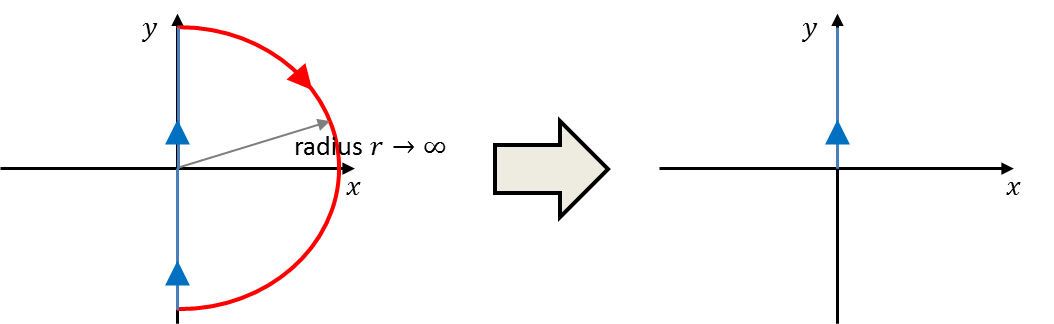
\includegraphics[width=0.9\linewidth]{Afbeelding12}
\end{itemize}
\end{frame}

\begin{frame}
\frametitle{Nyquist plot}
\begin{itemize}
\item Extracting the number of times ($-1$,$0$) is circled now isn't that difficult anymore:
\\ \begin{itemize}
\item You search for the image of $j0^+$
\item You search for the image $j\infty$
\item then you serach for the positive real y for which f(jy)'s imaginary part changes sign
\end{itemize}
\item This information allows you to determine if you encircle ($-1$,$0$)
\item Let’s show this with a simple example, but of course you can use software to do this! (e.g. nyquist in Matlab)
\end{itemize}
\end{frame}

\begin{frame}{Nyquist plot: a simple example}
\begin{itemize}
\item Let’s take the following open loop system:
\\ $P(s)C(s) = \frac{1}{s^2-2s+2}$
\item Fill in $s =j\omega \rightarrow \frac{1}{-\omega^2 -2j\omega +2} = \frac{1}{-\omega^2 +2 -2j\omega}\frac{-\omega^2 +2 +2j\omega}{-\omega^2 +2 +2j\omega}= \frac{-\omega^2+2+2j\omega}{(-\omega^2+2)^2+4\omega^2}$
\begin{itemize}
\item $f(j0^+) = \frac{1}{2}$
\item $f(j\infty) = 0 $
\item Imaginary part: $\frac{2\omega}{(-\omega^2+2)^2+4\omega^2}=0 \Rightarrow \omega = 0$
\end{itemize}
\item The real axis get's crossed $2$ times; first at $\frac{1}{2}$ ($\omega = 0^+$) an then at $0$ ($\omega = \infty$)$\rightarrow$ ($-1$,$0$) is not encircled
\end{itemize}
\end{frame}

\begin{frame}{Nyquist plot: a simple example}
\begin{itemize}
\item Remember our open loop system: $P(s)C(s) = \frac{1}{s^2-2s+2}$
\item $Z$ and $P$ are the number of zeros and poles of $1+P(s)C(s)$
\item The poles of $P(s)C(s)$ and $1+P(s)C(s)$ are the same ($P=2$ in our example)
\item Since ($-1$,$0$) is not encircled: $Z-P=0$; hence there are $2$ zeros in the right half plane
\item Remember that the zeros of $1+P(s)C(s)$ are the poles of the closed loop system and thus, the unity feedback controller is unstable
\end{itemize}
\end{frame}

\begin{frame}{Nyquist plot: poles on the imaginary axis}
\begin{itemize}
\item There is one more thing to know about Nyquist plots: how to deal with poles on the imaginary axis
\item Why are they a problem?
\\ \begin{itemize}
\item Take for instance the case with one pair of imaginary poles at $jc$ and $-jc$
\item When coming close to $jc$ the argument will remain $0$ and the gain will increase to infinity
\item At $jc$ itself the gain will be infinite, but the argument is undetermined, hence we cannot map this point
\\ 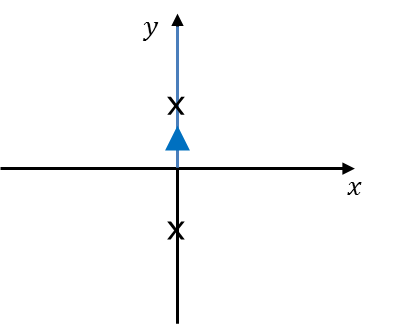
\includegraphics[width=0.5\linewidth]{Afbeelding13}
\end{itemize}
\end{itemize}
\end{frame}

\begin{frame}{Nyquist plot: poles on the imaginary axis}
\begin{itemize}
\item How do you solve this?
\begin{itemize}
\item Instead of going through the poles, we will evade them by an infinitesimally small amount (see figure)
\item That way we do not have the problem of an undetermined mapping at the pole
\item Since we avoid them by an infinitesimally small amount we also know we will not wrongly avoid a pole that lies in the right half plane
\\ 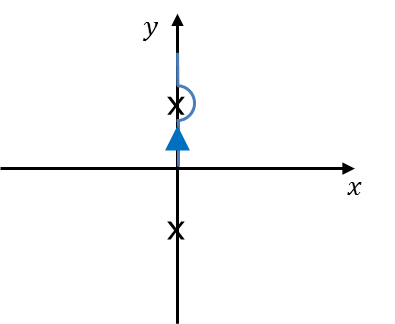
\includegraphics[width=0.4\linewidth]{Afbeelding14}
\end{itemize}
\item Now the Nyquist plot will go to infinity as $x$ is approached, then the argument will change from $0$ to $\pi$ as the semi-circle is traversed and then the Nyquistplot will return from infinity
\end{itemize}
\end{frame}

\begin{frame}{The Nyquist criterion in the discrete time case}
\begin{itemize}
\item The Cauchy argument principle still applies, since $P(z)C(z)$ also has the shape of a rational polynomial
\item The contour now will have to encircle the entire complex plane except for the unity circle
\\ 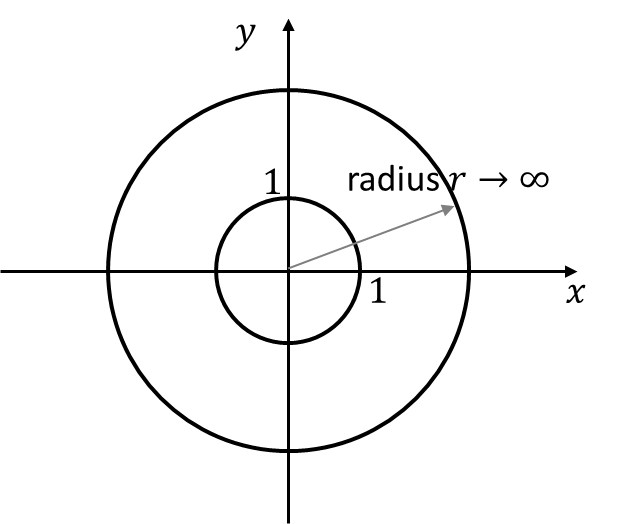
\includegraphics[width= 0.7\linewidth]{Afbeelding15}
\end{itemize}
\end{frame}

\begin{frame}{The Nyquist criterion in the discrete time case}
This is not a contour however, but this can be solved with the following trick:
\\ The two horizontal pieces are both infinitely close to the real axis, that way they are identical but with 	opposite signs. They will cancel each other.
\\ 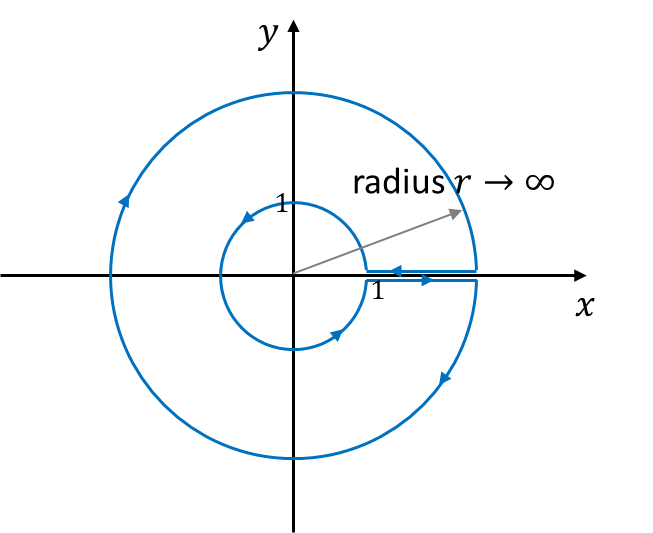
\includegraphics[width= 0.7\linewidth]{Afbeelding16}
\end {frame}

\begin{frame}{Margins}
\begin{itemize}
\item The Nyquist plot allows us to determine ‘how stable’ the system will be
\item We know that the stability changes when $1+P(s)C(s)$ has an imaginary zero (then the system is marginally stable)
\item Can we see such a zero in the Nyquist plot of $P(s)C(s)$?
\item Of course: the Nyquist plot is the image of the imaginary axis, so if there is a zero on the imaginary axis, the Nyquist plot of $1+P(s)C(s)$ would go through $0$ and the Nyquist plot of $P(s)C(s)$ will go through $-1$
\item Hence the system is marginally stable if the Nyquist plot goes through $-1$
\end{itemize}
\end {frame}

\begin{frame}{Margins}
\begin{itemize}
\item This explains why we can use the 'distance to $-1$' as a measure of stability
\item We will see two different stability margins, which can be easily read off the Nyquist diagram:
\begin{itemize}
\item The gain margin: the amount of extra gain you can allow before instability occurs (in dB)
\item The phase margin: the amount of phase you can add before instability occurs
\\ 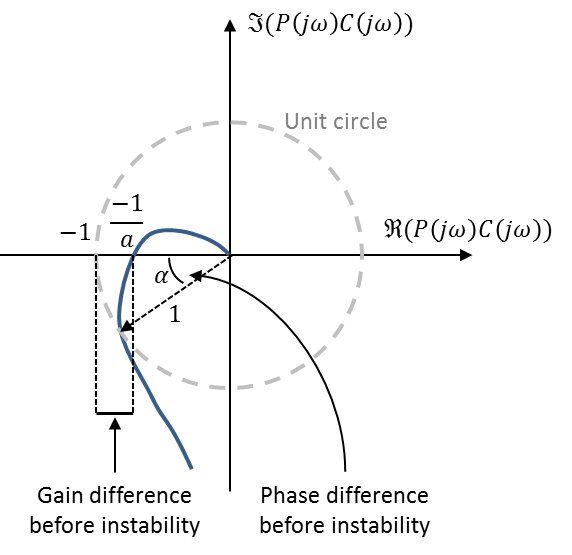
\includegraphics[width= 0.4\linewidth]{Afbeelding17}
\\ 
\includegraphics[width=0.4\linewidth]{Afbeelding18}
\end{itemize}
\end{itemize}
\end {frame}

\begin{frame}{Margins: gain margin}
\begin{itemize}
\item The gain margin is the amount of extra gain allowed before the system becomes unstable
\item Or: how much larger the gain has to be, before the system becomes unstable
\item The gain margin is \textbf{multiplicative}, so it is the factor with which you have to multiply the gain so the Nyquist plot goes through $-1$ in the\\𝑤$w$-plane
\item It will be expressed in dB; take $K$ a certain factor, then this can be expressed in dB: $20.log_{10} K$ dB 
\end{itemize}
\end {frame}

\begin{frame}{Margins: gain margin}
\begin{itemize}
\item Let’s look at this the following way:
\\ 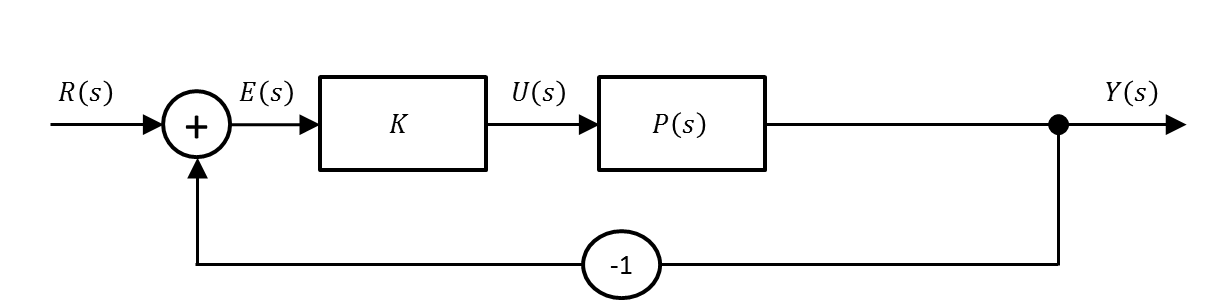
\includegraphics[width=0.9\linewidth]{Afbeelding19}
\item The stability margin of $P(s)$ with unity feedback is the $K$𝐾for which the system above is marginally stable
\end{itemize}
\end {frame}

\begin{frame}{Margins: gain margin}
\begin{itemize}
\item So $KP(s)$ should equal $-1$ for an imaginary $s=j\omega$
\item This requires $\angle(KP(j\omega)) = \angle P(j\omega)$ to equal $-180^{\circ}$ ; this $ \omega_\pi $𝜋is called the gain crossover frequency (GCF)
\item $K$ then has to be set such that $|KP(j\omega_\pi)|=1 $
\item So now you should be able to understand that a large gain can lead to instability; and that this risk only exists when there exists a $\omega_\pi$ for which $\angle P(j\omega)= -180°$
\item We will illustrate this with a few examples
\end{itemize}
\end {frame}

\begin{frame}{Margins: gain margin examples}
\begin{itemize}
\item Take $ P(s) = \frac{1}{s(s+2)} $
\item $\angle P(j\omega) = -tan^{-1}(\frac{\omega}{0}) -tan^{-1}(\frac{\omega}{2}) = -90^{\circ} - tan^{-1}(\frac{\omega}{2})$
\item So when is this equal to $-180^{\circ} $ ?
\item This would require $\omega \rightarrow \infty $
\\ which makes $P(j\omega)=0$
\item So the gain margin is infinite in this case
\end{itemize}
\end {frame}

\begin{frame}{Margins: gain margin examples}
\begin{itemize}
\item We will show this again in the Nyquist plot:
\\ 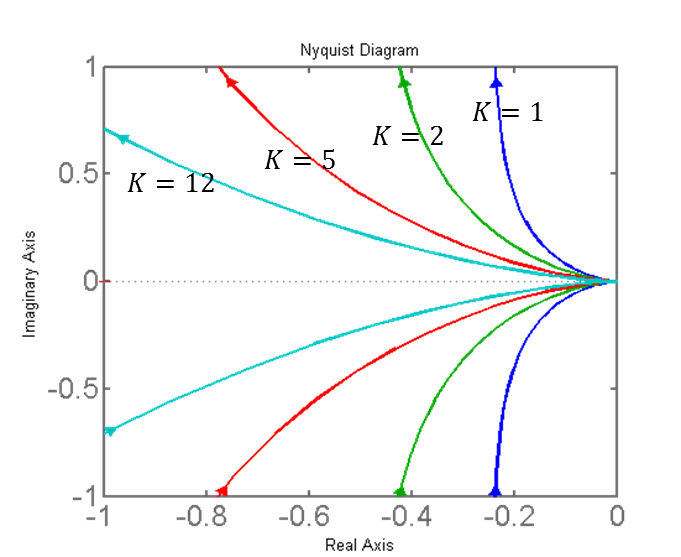
\includegraphics[width=0.7\linewidth]{Afbeelding20}
\item The only crossover with the real axis is at $\omega=0$ and that doesn't change with increasing $K$𝐾
\end{itemize}
\end {frame}

\begin{frame}{Margins: phase margin}
\begin{itemize}
\item The phase margin is how much you can rotate the Nyquist diagram before $-1$ is crossed
\item This can be interpreted as multiplying $P(s)$ with $e^{j\theta}$ until $-1$ is crossed
\item So $P(s)e^{j\theta} = -1$ for an imaginary $s=j\omega$
\item This requires $|P(j\omega)e^{j\theta}| = |P(j\omega)|$ to equal 1; this $\omega_0$ is called the Phase Crossover Frequency (PCF)
\item $|\theta|$ then has to be set such that $\angle(P(s)e^{j\theta}) = \angle P(s) +\theta = -180^{\circ}$
\item The gain margin is defined as positive, but that doesn’t matter, because of the symmetry with respect to the real axis: 
\\If a rotation of $\theta$ degrees results in a crossing of $-1$, then a rotation of $-\theta$ does the same  
\end{itemize}
\end {frame}

\begin{frame}{Margins: phase margin}
\begin{itemize}
\item Let’s take $P(s) = \frac{1}{s(s+2)}$ again
\item When is $|P(j\omega)|=1$ ?
\\ $\frac{1}{\omega}.\frac{1}{\sqrt{\omega^2+4}} =1$, hence $\sqrt{\omega^4+4\omega^2}=1$, or $\omega= \sqrt{\sqrt{5}-2}=0.486$
\item Find $\theta$ so $\angle (P(j\omega)e^{j\theta}) = -180^{\circ}$
\item $\theta = -180^{\circ} + tan^{-1}(\frac{\omega}{0}) + tan^{-1}(\frac{\omega}{2}) = -76.34^{\circ}$ \\The phase margin is $76.34^{\circ}$
\end{itemize}
\end {frame}

\begin{frame}{Margins: phase margin}
We’ll show this graphically with the Nyquist plot:
\\ 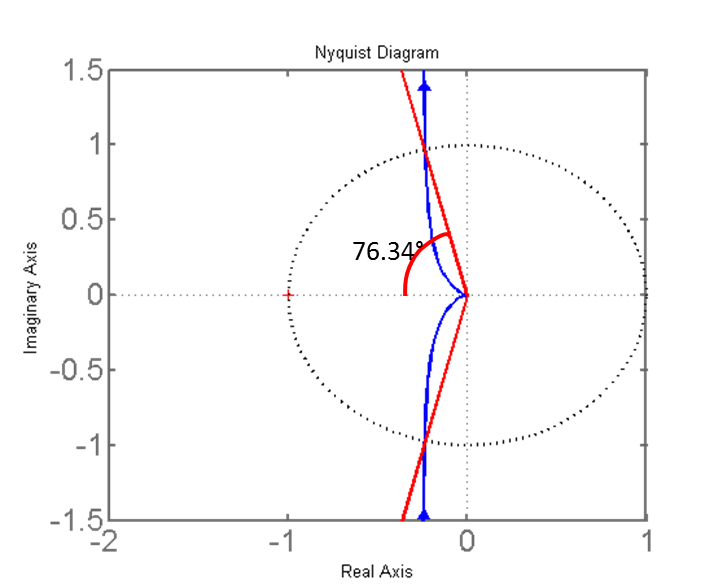
\includegraphics[width= 0.7\linewidth]{Afbeelding21}
\end {frame}

\begin{frame}{Margins: what should the margins be?}
Phase margin:
\begin{itemize}
\item This is more subtle than the gain margin
\item If it is too small instability might occur due to practicalities
\item If it is too small we get large overshoots and large oscillations that fade away very slowly(which is not something we associate with a good form of stability)
\item Sometimes a good value is $60^{\circ}$, but it is highly case dependent
\end{itemize}
A good margin does not offer certainty about the stability; whereas a bad phase margin (very large or very small) does give certainty about instability
\end {frame}

\begin{frame}{Margins using Bode plots}
We can also easily derive the gain and phase margins from the Bode plots of $P(s)C(s)$:
\\ 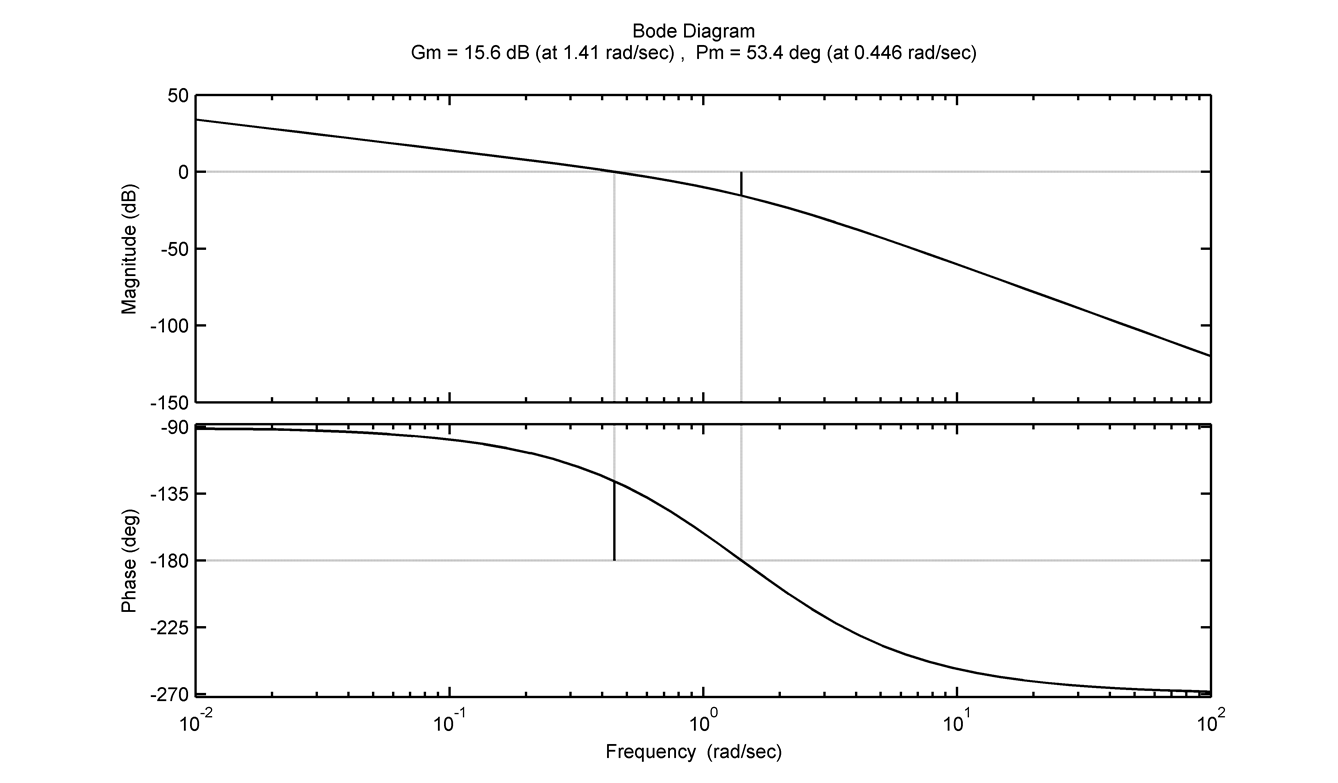
\includegraphics[width=1.1\linewidth]{Afbeelding22}
\end {frame}

\begin{frame}{Margins: design example}
\begin{itemize}
\item We’ll design a simple proportional controller for the system $P(s) = \frac{1-s}{(1+s)^2}$ 
\\ 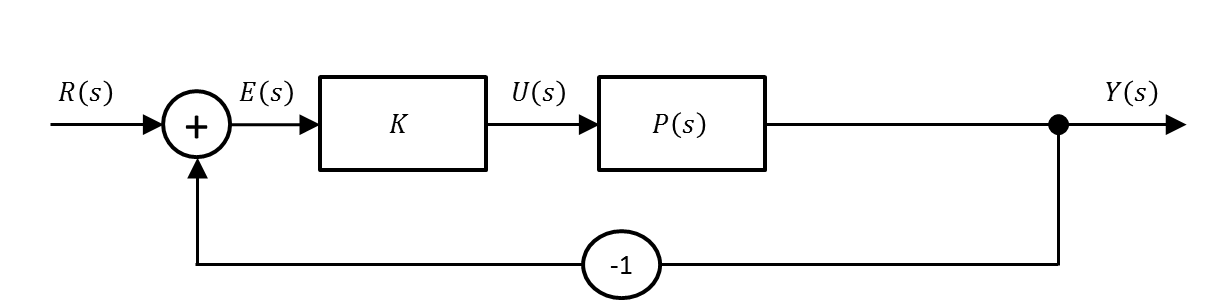
\includegraphics[width=0.8\linewidth]{Afbeelding19}
\item What will $K$ have to be in order to have a phase margin of $45^{\circ}$ ?
\end{itemize}
\end {frame}

\begin{frame}{Margins: design example}
\begin{itemize}
\item We find $\omega$ by setting $\angle(P(j\omega)e^{\frac{j\pi}{4}})= -180^{\circ}$
\begin{itemize}
\item $45^{\circ} + tan^{-1}(-\omega)-tan^{-1}(\omega)-tan^{-1}(\omega) = -180^{\circ}$
\item $-3tan^{-1}(\omega)=-225^{\circ}$
\item $\omega = tan(75^{\circ})=3.73$
\end{itemize}
\item Now we can find $K$ (which doesn't influence the argument) by setting $|KP(j\omega)|=1$ :
\\ $K\frac{\sqrt{\omega^2+1}}{\sqrt{\omega^2+1}^2} = \frac{K}{\sqrt{\omega^2+1}} = \frac{K}{3.86} = 1$ $\rightarrow$ $K=3.86=5.87$dB
\end{itemize}
\end {frame}

\begin{frame}{Margins: design example}
\begin{itemize}
\item We can do this graphically with the Nyquist plot
\item First determine the point that corresponds to $\theta = 45^{\circ}$
\item Then determine the modulus;
\\ $K$ is then equal to the inverse of that modulus
\\ 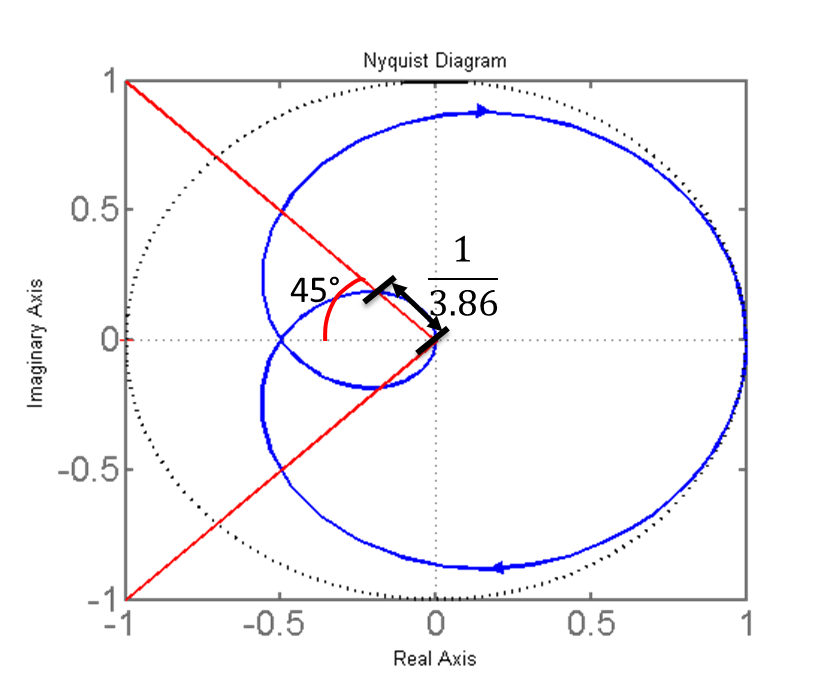
\includegraphics[width=0.7\linewidth]{Afbeelding23}
\end{itemize}
\end {frame}

\begin{frame}{Let's recapitulate}
\begin{itemize}
\item The Nyquist stability criterion came to existence as a cheap alternative to determine stability of a closed loop system with unity feedback
\item It also allows to see the phase margin and the gain margin; which are used to measure how stable the system actually is 
\item It’s relevance today is as a design tool, as shown in the final example
\item In the next section we will discuss new kinds of classical control components 
\item Bode plots make up a similar tool, yet the Nyquist stability criterion is (slightly) more generally applicable
\end{itemize}
\end {frame}

\begin{frame}{Interesting links}
\begin{itemize}
\item About the Nyquist argument principle:
\begin{itemize}
\item \url{https://www.youtube.com/watch?v=sof3meN96MA&index=3&list=PLEJyHgf7y0ie3nwSzMDVzAdxf4dK9m89a}
\item \url{https://www.youtube.com/watch?v=tsgOstfoNhk
}
\end{itemize}
\item About margins:
\begin{itemize}
\item \url{https://www.youtube.com/watch?v=Hw_hrxsX4_M
}
\item \url{https://www.youtube.com/watch?v=BTNZ8SRs7Y8
}
\item \url{https://www.youtube.com/watch?v=V1mfy7VhJNQ
}
\end{itemize}
\end{itemize}
\end {frame}

